\documentclass[10pt,a4paper]{article}
\usepackage[margin=1.95cm,top=2.2cm,bottom=2.05cm]{geometry}
\usepackage[T1]{fontenc}
\usepackage{lmodern,microtype,booktabs,tabularx,array,graphicx,xcolor}
\usepackage{enumitem,caption,fancyhdr,xurl,float,amsmath,needspace}
\usepackage[unicode,colorlinks=true,urlcolor=blue!65!black,linkcolor=black]{hyperref}
\graphicspath{{../analysis/figures/}}
\definecolor{ink}{HTML}{202A32}\definecolor{navy}{HTML}{173E56}
\definecolor{muted}{HTML}{586974}\definecolor{rule}{HTML}{CED8DD}
\color{ink}\setlength{\parindent}{0pt}\setlength{\parskip}{0.30em}
\newcolumntype{Y}{>{\raggedright\arraybackslash}X}
\newcolumntype{P}[1]{>{\raggedright\arraybackslash}p{#1}}
\setlength{\emergencystretch}{2em}\renewcommand{\arraystretch}{1.18}
\captionsetup{font=small,labelfont=bf}\setlist[itemize]{leftmargin=1.25em,itemsep=.1em,topsep=.15em}
\pagestyle{fancy}\setlength{\headheight}{22pt}\fancyhf{}
\fancyhead[L]{\footnotesize\color{muted} IIB423T-1 / Workshop 2}
\fancyhead[R]{\footnotesize\color{muted} Medina \& Castillo}
\fancyfoot[R]{\footnotesize\color{muted}\thepage}\renewcommand{\headrulewidth}{.35pt}
\newcommand{\sectionhead}[1]{\Needspace{8\baselineskip}\vspace{.4em}{\large\bfseries\color{navy}#1}\par\vspace{.1em}}
\newcommand{\subhead}[1]{\vspace{.2em}{\bfseries #1}\par}
\begin{document}\thispagestyle{empty}
{\small\bfseries\color{navy} BUSINESS INTELLIGENCE / WORKSHOP 2}\par\vspace{.6em}
{\LARGE\bfseries Customer concentration: from EDA to credible validation}\par\vspace{.35em}
{\large A descriptive validation and sampling study of UCI Online Retail}\par\vspace{.5em}
{\color{muted}Mois\'es Medina and Ignacia Castillo\hfill 20 October 2026}\par
\vspace{.6em}{\color{rule}\hrule height .65pt}\vspace{.6em}
\textbf{Submission role.} This is a supplemental report. The primary W2 evidence is the executable English notebook \path{notebooks/W2_project.ipynb}, with saved outputs, data and execution instructions in the GitHub repository. The specific W2 brief sets the deadline at 29 October 2026, 23:59, Chile. Its printed release date is 22 October; that header is not a claim about when this work was performed.

\sectionhead{1\quad Continuity, decision and measurement}
We retain the W1/C1 question: how much eligible recorded purchase value is attributable to the highest-value 10\% of identifiable customers, and how much value cannot enter that ranking because an ID is missing? A proposed commercial analyst could use the evidence for a retrospective account review and a review of ID capture. This is a proposed use, not the anonymous retailer's documented strategy.

The team reports 100/100 in C1. No specific instructor correction text was supplied for this stage. We therefore identify self-audits and new W2 extensions explicitly; a new validation requirement is not presented as proof that C1 was incorrect. The original W1/C1 submissions are preserved under \path{assessments/}.

Let $v_i$ denote eligible recorded value for known customer $i$, $N$ the known-ID population and $k=\lceil0.10N\rceil$. Sorting $v_i$ from highest to lowest,
\[
K_{10}=100\frac{\sum_{i=1}^{k}v_i}{\sum_{i=1}^{N}v_i},\qquad
C_{ID}=100\frac{\text{known-ID eligible value}}{\text{all eligible purchase value}}.
\]
Values use pounds sterling; both measures are percentages. Cutoffs round upward to whole IDs. ID coverage is value-weighted, not a fraction of rows. Neither measure is net revenue, margin, loyalty, lifetime value or an established risk tolerance.

\begin{tabularx}{\linewidth}{@{}YY@{}}
\toprule
\textbf{Reproduced C1 baseline} & \textbf{W2 result} \\ \midrule
Source invoice lines & 516,384 \\
Eligible positive purchase lines & 500,531 \\
Identifiable customers / top-decile IDs & 4,293 / 430 \\
K10 / ID-value coverage & 60.5001\% / 85.6628\% \\
Eligible value / known-ID value & \pounds{}9,610,990.56 / \pounds{}8,233,040.56 \\
\bottomrule\end{tabularx}

The baseline matches C1 numerically within the executable floating-point tolerance. We retain its bounded concentration conclusion. W2 strengthens the checkable evidence and the interpretation of coverage and validation; it does not establish a current operational effect.
\clearpage
\sectionhead{2\quad Source, dictionary and analytical scope}
UCI Online Retail (Chen, 2015; DOI 10.24432/C5BW33; CC BY 4.0) describes an online gift retailer based in the UK with many wholesale customers. Its original file has 541,909 records from 1 December 2010 to 9 December 2011. The unchanged case input keeps all 516,384 rows through 30 November 2011, excluding only the final nine-day December fragment. Complete months have unequal lengths and activity; complete date coverage does not prove complete capture of real transactions.

One row is one recorded invoice line. An invoice contains multiple lines and a CustomerID can link multiple invoices. InvoiceNo is therefore not a unique row key. A C prefix identifies a cancellation record; there is no verified original-purchase link. Country is a label on the record, not a verified delivery destination or a necessarily stable attribute of an ID.

{\small
\begin{tabularx}{\linewidth}{@{}YYY@{}}
\toprule
\textbf{Original field} & \textbf{Meaning / unit} & \textbf{Type and missingness} \\ \midrule
InvoiceNo & Invoice identifier; C prefix marks a cancellation record & string; Not expected; cannot identify invoice if absent \\
StockCode & Source item/special-code identifier, not commercial category & string; Not expected; flag rather than invent item \\
Description & Recorded item description & nullable string; Unknown/unrecorded description; not proof of zero activity \\
Quantity & Signed units on an invoice line & integer; Not expected; cannot calculate line value \\
InvoiceDate & Recorded invoice-line timestamp & datetime; Not expected; cannot assign period \\
UnitPrice & Recorded unit price in GBP & numeric; Not expected; no price imputation \\
CustomerID & Identifier linking recorded lines to a customer account & nullable integer; Unidentified purchase; no ID imputation \\
Country & Customer country recorded on this line & string; Meaning unknown if absent; not delivery destination \\
\bottomrule\end{tabularx}
}

The full machine-readable dictionary also covers derived flags, source row, row groups, split membership, value and KPI formulas.\par
\textbf{Eligibility.} A purchase must have positive Quantity and UnitPrice, no C prefix and a StockCode matching five digits with an optional final letter. The pattern is a provisional scope rule, not a verified commercial classification. Eligible line value is Quantity times UnitPrice. Eligible cancellation records instead require a C prefix, negative quantity, positive price and the same code rule. All remaining rows stay in the prepared file outside both measures.

\textbf{Retention rationale.} A missing ID prevents ranking but does not erase recorded value. A missing description alone does not affect the calculation. A zero or negative price is outside the positive-value measure; substituting another price would invent a charge without knowing the reason. Exact repeats remain in the baseline because no source-line identifier establishes which are erroneous. We test alternatives instead of silently deleting records. An undefined derived value outside the purchase scope is not an observed zero.

\begin{tabularx}{\linewidth}{@{}YY@{}}
\toprule
\textbf{Mutually exclusive group} & \textbf{Rows} \\ \midrule
other\_retained & 7,502 \\
priced\_C\_record & 8,351 \\
priced\_purchase & 500,531 \\
\bottomrule\end{tabularx}

The input SHA-256 is checked before analysis. Original fields and the one-to-one source-row identifier are preserved in the prepared table. No source lines are lost; flags may overlap, whereas the three row groups do not.
\clearpage
\sectionhead{3\quad Quality validation and consequential checks}
The notebook implements seventeen checks. Structural violations stop execution; scoped exceptions are flagged with a documented treatment. ``Flag'' does not mean the record has been proved wrong. The source and prepared counts both remain 516,384.

{\small
\begin{tabularx}{\linewidth}{@{}P{.43\linewidth}P{.15\linewidth}Y@{}}
\toprule
\textbf{Check} & \textbf{Count / status} & \textbf{Treatment} \\ \midrule
Q01 Schema and numeric/time types & 0 / PASS & retain \\
Q02 Invalid/missing timestamps or outside case bounds & 0 / PASS & retain \\
Q03 Missing invoice or item identifier & 0 / PASS & retain \\
Q04 Nonpositive unit prices & 2,463 / FLAG & retain source; exclude from positive-value measures \\
Q05 Nonpositive quantities & 10,234 / FLAG & retain; separate eligible negative C records \\
Q06 Missing CustomerID & 127,216 / FLAG & retain eligible value; exclude from customer rank \\
Q07 Missing description & 1,439 / FLAG & retain if otherwise eligible \\
Q08 Exact repeated rows beyond first copy & 4,989 / FLAG & retain baseline; compare deduplicated sensitivity \\
Q09 Outside provisional merchandise-code pattern & 5,072 / FLAG & retain source; exclude baseline; test alternative patterns \\
Q10 Negative quantity without C prefix & 1,306 / FLAG & retain outside both eligible measures \\
Q11 Source-row conservation and disjoint partition violations & 0 / PASS & retain \\
Q12 Eligible purchase invoices with multiple known IDs & 0 / PASS & retain \\
Q13 Invoice numbers with multiple timestamps & 43 / FLAG & retain; use min/max interval and check split boundaries \\
Q14 Customer IDs with multiple country labels & 8 / FLAG & retain country at line level; flag identity consistency \\
Q15 Invoices crossing chronological partition boundaries & 0 / PASS & retain \\
Q16 Missing quantities or prices & 0 / PASS & retain \\
Q17 Purchase invoices mixing identified and unidentified lines & 0 / PASS & retain \\
\bottomrule\end{tabularx}
}

Invoice timestamps vary within 43 InvoiceNo values; the maximum observed span, in minutes, is 1, and 0 of these intervals cross a calendar day. We preserve original timestamps and use first/last times to verify boundaries. None crosses the specified train/validation/test boundaries. Eight IDs have multiple country labels. We retain country at line level rather than asserting fixed residence or overwriting an ID's history. Exception tables list the affected identifiers and evidence.

\clearpage
\sectionhead{4\quad Feedback-to-action and changes to conclusions}
The entries below are self-audits or W2 extensions. They are not attributed to the instructor. The full table includes notebook sections, generated evidence paths and the reason for each action.

{\small
\begin{tabularx}{\linewidth}{@{}YYY@{}}
\toprule
\textbf{Issue} & \textbf{Action} & \textbf{Consequence} \\ \midrule
A provisional product-code scope could be mistaken for a verified category & Keep the rule explicit and repeat narrow/broad code sensitivities & K10 is conditional on the stated merchandise rule \\
43 invoices have multiple timestamps & Inspect first/last timestamps and assert no invoice crosses split boundaries & Retain invoice lines; do not assign future lines to an earlier partition \\
8 CustomerIDs have multiple country labels & Keep source country per line; use line-value country proportions; do not force one country per ID & Country comparisons do not establish fixed residence or stable identity \\
K10 monthly ranking changes with observed IDs and coverage & Show monthly N and ID-value coverage alongside K10 & A lower K10 alone does not establish diversification \\
Entire source period was explored in W1/C1 & Freeze W2 rules and use chronological held periods with prior-exposure disclosure & No predictive-accuracy or virgin-holdout conclusion \\
\bottomrule\end{tabularx}
}

\subhead{What changed and what did not}
The numerical full-case K10 and coverage remain unchanged. The product-code interpretation is made explicitly provisional. Invoice time and country consistency receive new executable checks. The monthly narrative states that population mix and missingness are possible explanations, rather than claiming a causal mechanism. The temporal holdout is documented as reused historical evidence because W1/C1 already inspected all periods. No claim of predictive performance is added.

\subhead{Five Cs carried forward}
Clean: observable checks and justified retention are exported. Consistent: unchanged purchase and KPI rules apply across the twelve months. Conformed: no external join is forced; cross-source agreement is not applicable. Current: 2010--2011 records support historical analysis; recent data are needed for operational use. Comprehensive: unidentified value, provisional product scope, missing financial costs/payments and absent purchase--cancellation links remain limitations.
\clearpage
\sectionhead{5\quad Revised exploratory evidence}

\begin{figure}[H]\centering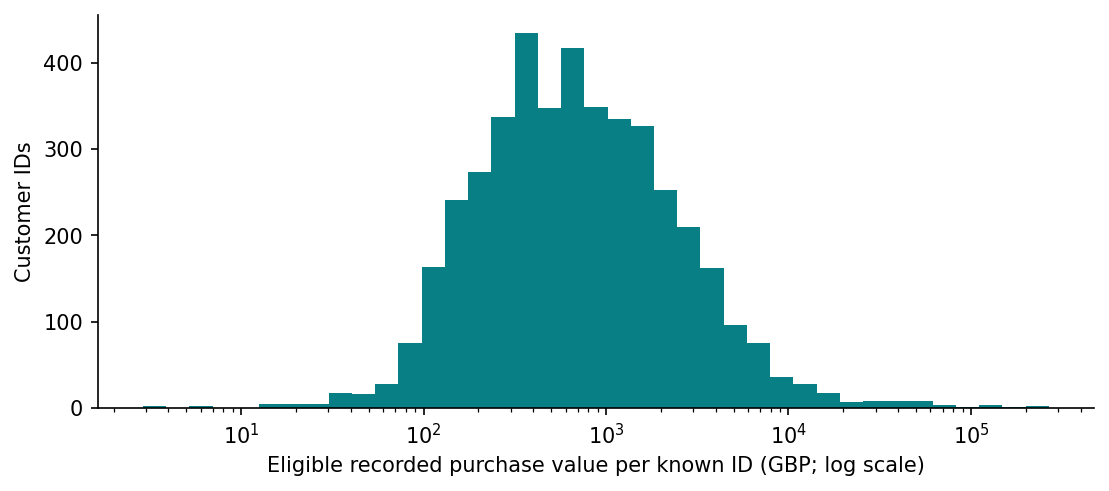
\includegraphics[width=.95\linewidth]{customer_value_distribution.png}\caption{Known-ID eligible purchase value over the full twelve-month case. The logarithmic x-axis makes the long upper range visible; it does not remove large accounts.}\end{figure}

The median is \pounds{}652.80, the mean \pounds{}1,917.78, and the maximum \pounds{}267,410.00. The mean is not representative of every customer. A large recorded account is not, by itself, proof of an error or of loyalty.

\begin{figure}[H]\centering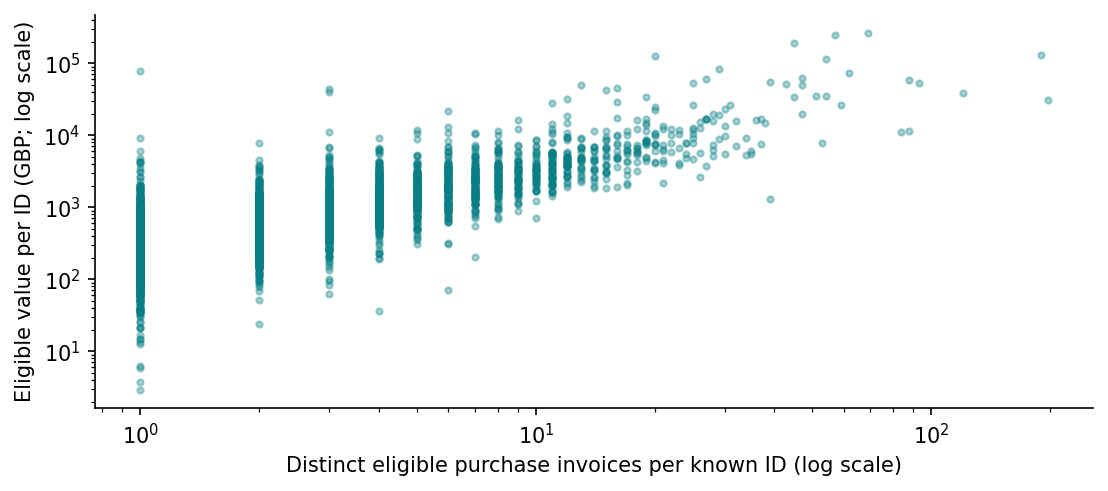
\includegraphics[width=.95\linewidth]{frequency_value_relationship.png}\caption{Eligible invoice frequency and recorded value per known ID. Both axes use logarithms; each point is a known customer in this window.}\end{figure}

Spearman correlation is 0.803; Pearson correlation is 0.569. More observed invoices give more opportunities to accumulate value, so the relationship is partly arithmetic. It does not establish that an intervention would cause higher loyalty, revenue or profit.

\clearpage

\begin{figure}[H]\centering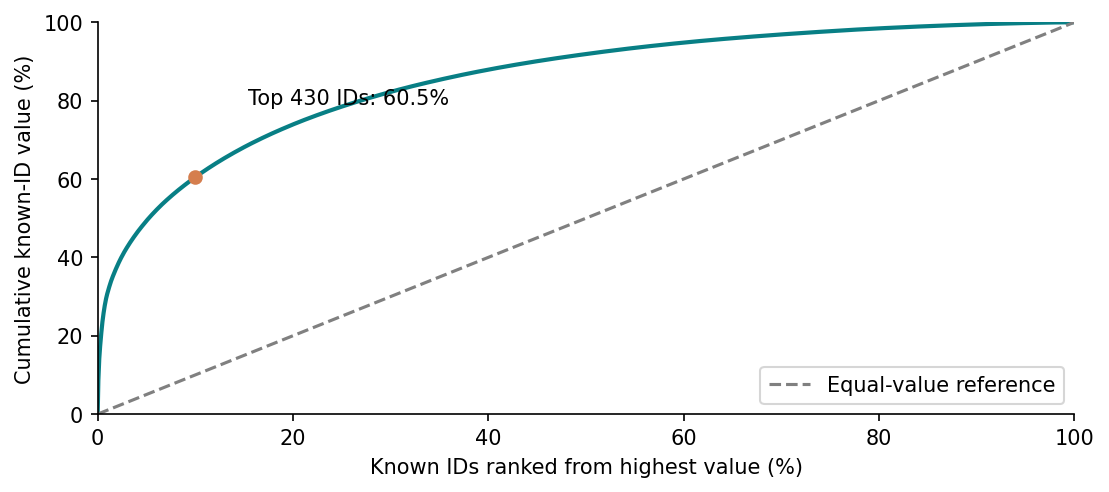
\includegraphics[width=.95\linewidth]{concentration_curve.png}\caption{Cumulative known-ID value ranked from highest to lowest; the diagonal is an equal-value reference. The top group is rounded to 430 IDs.}\end{figure}

The top 430 of 4,293 identified customers account for 60.5\% of known purchase value. This concentration is conditional on IDs covering 85.7\% of all eligible value. Sensitivity checks give K10 between 59.22\% and 60.58\%; they do not recover unidentified purchases.

\begin{figure}[H]\centering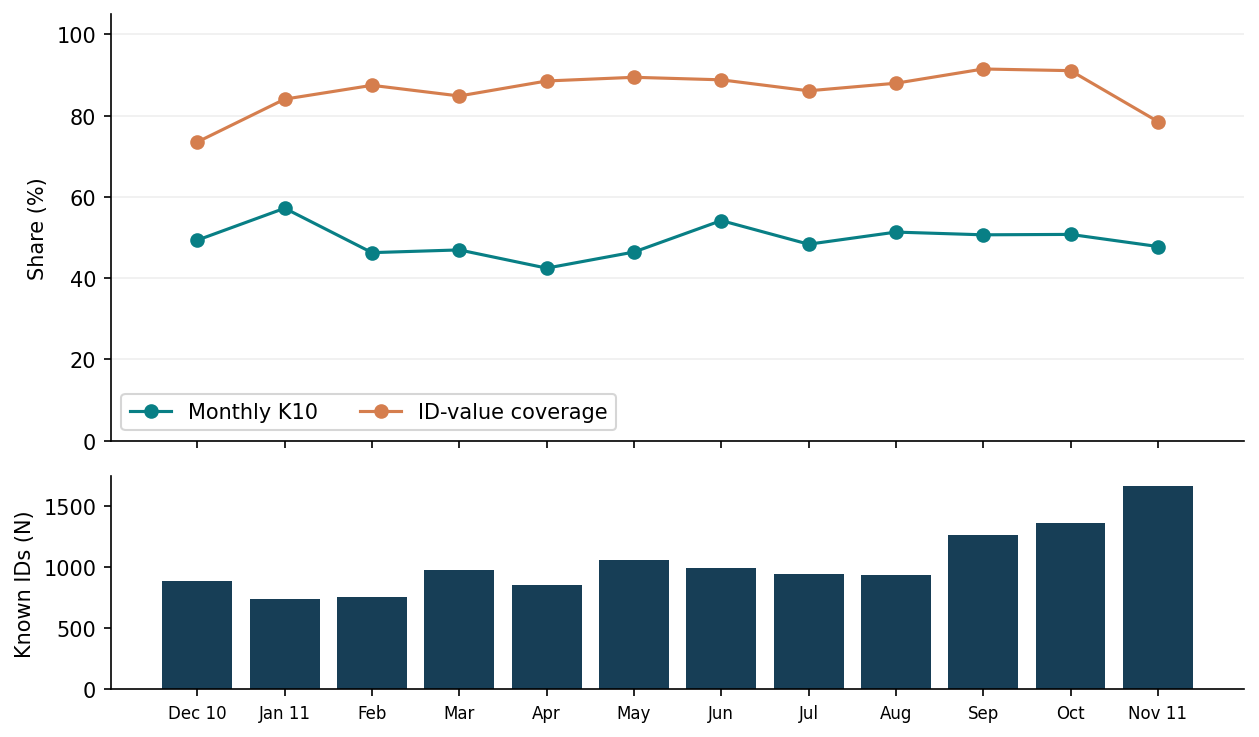
\includegraphics[width=.95\linewidth]{monthly_kpi_coverage_population.png}\caption{Monthly K10 and ID-value coverage share a 0--100 percent scale; the lower panel reports known-ID population N. IDs are re-ranked within each month.}\end{figure}

October K10 is 50.8\% and November K10 47.8\%, while ID coverage falls from 91.1\% to 78.6\%. This does not establish diversification or prove that missing IDs caused the change. Different account mixes, identification processes and activity could affect the observed ranking. One annual cycle cannot establish a recurring Christmas effect.
\clearpage
\sectionhead{6\quad Sampling and representativeness}
The historical target is relevant purchase activity for the retailer during the selected year. The observed population consists of the available source records within our complete-month extract. The value dataset includes eligible purchase lines; K10 additionally requires identifiable customer aggregates. None is a probability sample of UK retailers. A future operational target would require recent accounts and processes.

Plausible coverage biases include unidentified purchases, unrecorded activity in the operational source, the single historical gift retailer and provisional item-code exclusions. Splitting records cannot repair these source-coverage mechanisms.

We select approximately 25\% of distinct invoices within each earliest-invoice-month, using seed 4232026 and whole-invoice rounding. All lines of selected invoices remain together. The size is an instructional subsampling exercise, not a claim of population power or precision. Varying invoice sizes and rounding make the realized row percentage slightly different. The seed is fixed; it is not selected to make the sample look representative.

\begin{tabularx}{\linewidth}{@{}YYYY@{}}
\toprule
\textbf{Measure} & \textbf{Complete case} & \textbf{Invoice sample} & \textbf{Difference} \\ \midrule
Source rows & 516,384 & 130,912 & 25.35\% of source rows \\
Known customers & 4,293 & 2,217 & Ranking population changes \\
K10 & 60.50\% & 54.01\% & -6.49 pp \\
ID-value coverage & 85.66\% & 85.21\% & -0.45 pp \\
UK share of eligible value & 84.62\% & 83.13\% & -1.49 pp \\
\bottomrule\end{tabularx}

UK share uses the recorded country of each eligible purchase line and includes unidentified value. It does not force a permanent country onto a customer. Invoice sampling reduces observed history per ID and removes some IDs entirely; the observed top decile therefore changes. Sample K10 is not an unbiased reconstruction guarantee for the full customer's annual portfolio. These differences describe one fixed sample, not confidence intervals or proof of sampling bias. The complete case remains our main descriptive population. Sampling is separate from the chronological split and is not used to decide which rows fit preprocessing.

{\small
\begin{tabularx}{\linewidth}{@{}YYY@{}}
\toprule
\textbf{Month} & \textbf{Invoices: available / sampled} & \textbf{Rows: available / sampled} \\ \midrule
2010-12 & 2,025 / 506 & 42,481 / 10,569 \\
2011-01 & 1,476 / 369 & 35,147 / 8,485 \\
2011-02 & 1,393 / 348 & 27,707 / 6,971 \\
2011-03 & 1,983 / 496 & 36,748 / 9,410 \\
2011-04 & 1,744 / 436 & 29,916 / 7,824 \\
2011-05 & 2,162 / 540 & 37,030 / 8,830 \\
2011-06 & 2,012 / 503 & 36,874 / 9,177 \\
2011-07 & 1,927 / 482 & 39,518 / 10,596 \\
2011-08 & 1,737 / 434 & 35,284 / 8,261 \\
2011-09 & 2,327 / 582 & 50,226 / 11,938 \\
2011-10 & 2,637 / 659 & 60,742 / 16,089 \\
2011-11 & 3,462 / 866 & 84,711 / 22,762 \\
\bottomrule\end{tabularx}
}

\clearpage
\sectionhead{7\quad Temporal holdout and validation procedure}
The proposed decision time is after month-end. Completed invoices up to the cut-off are available for account review. Full-year future totals and ranks would not be legitimate earlier-period features. We partition the complete source case, not its 25\% invoice sample. All row groups, including missing-ID and non-measure records, are saved in the actual split files.

First, October--November is reserved as test. The earlier December--September development pool is the initial training pool before validation is removed. Second, August--September is carved out of that pool as validation, leaving December--July for fitting. Validation contains no test rows. This hierarchy and its parent-relative proportions are exported in \path{data/processed/split_hierarchy.csv}.

\begin{tabularx}{\linewidth}{@{}P{.34\linewidth}rrrr@{}}
\toprule
\textbf{Partition / inclusive months} & \textbf{Source rows} & \textbf{Row share} & \textbf{Invoices} & \textbf{Eligible known IDs} \\ \midrule
train: Dec 2010--Jul 2011 & 285,421 & 55.27\% & 14,722 & 3,145 \\
validation: Aug--Sep 2011 & 85,510 & 16.56\% & 4,064 & 1,769 \\
test: Oct--Nov 2011 & 145,453 & 28.17\% & 6,099 & 2,405 \\
\bottomrule\end{tabularx}

The boundaries are 1 August, 1 October and 1 December 2011, with half-open intervals. Calendar duration is not an imposed 80/20 row ratio; activity differs across months. Structural checks confirm every source row belongs to one partition, no invoice crosses a boundary and no exact source-record hash appears in two partitions.

\begin{tabularx}{\linewidth}{@{}YYYY@{}}
\toprule
\textbf{Comparison} & \textbf{Source-row overlap} & \textbf{Invoice overlap} & \textbf{Known-ID overlap} \\ \midrule
train / validation & 0 & 0 & 1352 \\
train / test & 0 & 0 & 1566 \\
validation / test & 0 & 0 & 1156 \\
\bottomrule\end{tabularx}

Repeated customers are intentional for reviewing the same account population in later periods. The held periods are separate observations, but not independent new-customer samples. A new-customer generalization claim would require grouped validation. We use period-specific aggregates and explicitly report overlap instead of asserting customer independence.

\subhead{Training-only fitted operation}
For each eligible invoice we sum its positive purchase value, apply log1p and fit StandardScaler on training invoices only. Invoice value is available after completion for the stated review; it would not be a valid predictor of itself before purchase. No CustomerID or price is imputed. K10 continues to use original pounds, not scaled values.

\begin{tabularx}{\linewidth}{@{}YYYY@{}}
\toprule
\textbf{Partition} & \textbf{Eligible invoices} & \textbf{Mean scaled log value} & \textbf{SD scaled log value} \\ \midrule
train & 11,040 & -0.0000 & 1.0000 \\
validation & 3,157 & 0.1457 & 0.9591 \\
test & 4,756 & 0.0871 & 0.9672 \\
\bottomrule\end{tabularx}

The fitted mean is 5.508743 and scale 1.194544, estimated from 11,040 training invoices. The validation gate requires finite transformed values, positive eligible invoice totals, unique invoice keys and unchanged training parameters. Failure stops execution before test transformation. The ordered fit, validation gate and test transformation are exported in \path{data/processed/validation_execution.csv}. These are applicability checks; no predictive-performance target or test-driven tuning is introduced. Nonzero held-period means do not justify refitting on them.

\textbf{Exposure limit.} W1/C1 already inspected all twelve months. The protocol was fixed before W2 result tables, but the current holdout cannot become an untouched prospective test by relabeling it. It is a descriptive robustness comparison. We report monthly KPIs rather than interpreting unequal-duration partition totals as comparable. No predictive model, outcome label or accuracy metric is produced.
\clearpage
\sectionhead{7\quad Temporal holdout: descriptive findings}
After validation, we recalculate K10 and coverage separately within each month using only that month's purchases and known IDs. Each month receives equal weight in the summary below. These are means of monthly shares, not a pooled-period K10 or a comparison of raw totals from unequal windows.

\begin{tabularx}{\linewidth}{@{}YYYY@{}}
\toprule
\textbf{Partition / months} & \textbf{Mean monthly K10} & \textbf{Monthly K10 range} & \textbf{Mean monthly ID coverage} \\ \midrule
train / 8 & 48.91\% & 42.48\% -- 57.21\% & 85.34\% \\
validation / 2 & 51.01\% & 50.67\% -- 51.34\% & 89.72\% \\
test / 2 & 49.28\% & 47.79\% -- 50.77\% & 84.81\% \\
\bottomrule\end{tabularx}

Test mean monthly K10 differs from training by +0.37 percentage points. Concentration remains substantial in the held months, while its level varies. The annual K10 of 60.50\% pools longer customer histories; it is not a target expected in every month.

\textbf{Interpretation.} Observed customer mix, invoice histories and ID coverage differ between months. These descriptive differences do not identify a cause, establish a seasonal effect or measure predictive accuracy. The detailed monthly table includes each denominator and is saved as \path{data/processed/holdout_monthly_kpi.csv}.

\textbf{Audit amendment, 21 October 2026.} The explicit development hierarchy, ordered validation gate and this holdout table strengthen the evidence for criterion F. They preserve the previously fixed dates, eligibility and scaler. They were added after prior full-case exposure; no claim of newly unseen test data is made, and no observed difference selects a transformation or rule. A genuinely later period remains necessary for prospective evaluation.

\clearpage
\sectionhead{8\quad Context-specific leakage audit}
The audit reports observed risks, conditional future risks and implemented safeguards. Status is contextual: shared customer IDs do not alone imply inappropriate leakage for the same-account scenario, but invalidate an independent new-customer claim.

{\small
\begin{tabularx}{\linewidth}{@{}P{.23\linewidth}P{.27\linewidth}Y@{}}
\toprule
\textbf{Risk / status} & \textbf{Evidence} & \textbf{Consequence and mitigation} \\ \midrule
Future full-case customer totals/rank / present in prior artifacts & C1 aggregates span Dec 2010--Nov 2011; not W2 pre-cutoff features & Would reveal later purchases before review date. Rebuild invoice/period aggregates from rows available at that cut-off; exclude full-year rank from features \\
Repeated customer accounts / present & 1566 known IDs occur in both train and test & Invalid new-customer independence claim; global customer aggregation could leak future history. Allow repeated IDs for same-account time review; disclose dependence; no full-case profile reuse \\
Duplicated event lines across partitions / absent across chosen partitions & 4989 extra exact repeats within source; zero record-hash and invoice overlap across partitions & Random line splitting could put copies or sibling invoice lines on both sides. Partition by recorded time and verify invoice/record-hash boundaries; retain baseline repeats with sensitivity \\
Preprocessing learned on validation/test / absent in W2 & Scaler fit on 11040 train invoices; parameters unchanged after transformations & Full-data mean/scale would let held data influence fitted rule. Fit once on train; transform validation/test; export fit parameters and invariance checks \\
Target-derived variables in hypothetical prediction / uncertain for future use; no target/model in W2 & Invoice value, period value and K10 use completed purchases & Predicting the same purchase value from its total/rank would be circular. Define any future outcome and horizon first; use only prior-cutoff information; no accuracy claim here \\
Prior full-case exploration / analyst leakage / present & W1/C1 inspected all twelve months, including Oct--Nov; source snapshots retained & Current test cannot be described as untouched prospective evidence. Prespecify W2 transformations; treat as descriptive robustness; collect a genuinely later period before prospective evaluation \\
Linked external tables / absent / not applicable & Single UCI source; W2 performs no external join & Future joins could leak later customer states or create duplicate rows. No forced join; require as-of keys, cardinality and match checks before future integration \\
\bottomrule\end{tabularx}
}

A future predictive task must specify an outcome and horizon, and restrict inputs to what exists at the decision cut-off. Customer-profile clustering remains a possible later descriptive extension with no invented target labels. W2 establishes boundaries and a fitted transformation, not model feasibility or performance.
\clearpage
\sectionhead{9\quad Management summary}

Our historical account-review question and K10 definition remain unchanged from C1. The complete case still contains 4,293 identifiable customers: the highest-value 10\% account for 60.5\% of known purchase value, while IDs cover 85.7\% of eligible value. W2 adds explicit validation, a month-stratified invoice sample and chronological training, validation and test partitions. We retained 43 invoices with multiple timestamps and 8 IDs with multiple country labels, documenting their interpretation rather than overwriting records. The sample contains 25.4\% of source lines and yields K10 of 54.0\%, illustrating the effect of observing fewer invoices per customer. Train-only preprocessing prevents held periods from determining the fitted scale. However, missing IDs, provisional product codes and prior exploration of all periods still limit generalization. We recommend reviewing major accounts and ID capture together, then obtaining recent transactions and verified identity/code definitions before operational use or prospective evaluation.

\sectionhead{10\quad Process record and rubric evidence}
\subhead{Decisions and checks}
The unchanged input hash, source-row conservation, baseline reproduction, seventeen quality checks, whole-invoice sample, partition overlaps and scaler parameters are executable evidence. \path{evidence/protocol.json} records seed, row rules, time windows, exposure history and the no-test-tuning policy. The notebook is run from a fresh kernel with saved outputs. Exported tables and figures are regenerated from that same code; this report's numeric content is generated from those outputs.

\subhead{Feedback and contributions}
The team-reported C1 result is 100/100. No case-specific correction text is fabricated. Section 4 records five self-audit/extension entries. The members are Mois\'es Medina and Ignacia Castillo; no new individual task division or personal reflection has been invented for W2.

\subhead{AI use and verification}
OpenAI Codex assisted with code, notebook/report drafts and formatting. The implementation request prescribed continuity, invoice sampling, fixed seed, time partitions and a training-only scaler. Accepted suggestions include explicit flags and exported check evidence. Claims that zero prices have a proven discount cause, repeats are proven errors, C invoices establish matched returns, or the holdout is pristine are excluded. Assertions and automated reruns verify consequential suggestions. Those are automated checks, not claims that a particular student personally performed each check. The team is responsible for reviewing and defending the final analysis.

{\small
\begin{tabularx}{\linewidth}{@{}YY@{}}
\toprule
\textbf{W2 criterion} & \textbf{Inspectable evidence} \\ \midrule
A Continuity and feedback & Notebook 1--3; preserved assessments; feedback\_to\_action.csv; unchanged baseline \\
B Revised EDA & Notebook 4; four labelled figures; statistics, denominators and limits \\
C Validation & Notebook 2--3; dictionary; quality\_checks.csv; row\_flow.csv; exception tables \\
D Sampling & Notebook 5; sample\_strata.csv; actual sample; KPI/UK comparison and bias discussion \\
E Leakage & Notebook 7; seven contextual risks with evidence, status and safeguards \\
F Holdout and validation & Notebook 6; actual split files, counts, overlaps, fit parameters and prior-exposure limit \\
G Communication & Executed English notebook; README; summary; AI statement; repository commit/tag \\
\bottomrule\end{tabularx}
}

\clearpage
\sectionhead{References and source attribution}
\begin{enumerate}
\item Chen, D. (2015). \emph{Online Retail}. UCI Machine Learning Repository. DOI: \href{https://doi.org/10.24432/C5BW33}{10.24432/C5BW33}. Dataset/dictionary/licence: \url{https://archive.ics.uci.edu/dataset/352/online-retail}. CC BY 4.0. Original retrieval evidence remains in the preserved source manifest; W2 uses the unchanged local extract.
\item Fontecilla, T. (2026). \emph{Workshop 2: From Exploratory Analysis to Credible Validation}. Student brief and rubric supplied in the course workspace. Deadline printed: 29 October 2026.
\item Course notebooks (2026): \emph{Validation, Leakage and Reproducible Pipelines}; \emph{Guided Validation Case}; \emph{Sampling, Regression and Classification}. Used for split selection, leakage and training-only preprocessing. Course files are cited but not redistributed.
\item Medina, M., and Castillo, I. (2026). W1 and C1 submitted project reports and executed notebooks, preserved under \path{assessments/}. Prior concentration evidence and source limitations are retained for continuity.
\end{enumerate}
\end{document}
